\newpage
\chapter{ANEXOS}
%\addcontentsline{toc}{chapter}{ANEXOS}
\newpage
%\phantomsection
\section{PLAN DE GESTIÓN DE RIESGOS}\label{sec:plan-riesgos}
%\addcontentsline{toc}{section}{PLAN DE GESTIÓN DE RIESGOS}
La gestión de los riesgos consiste en la identificación de los riesgos y la planificación para minimizar su efecto en el proyecto. Siguiendo la metodología del PMBOK \cite{PMBOK}, se define una gestión compuesta por los siguientes pasos:
\begin{itemize}
\item Planificar la Gestión de Riesgos.
\item Identificar los riesgos.
\item Realizar el análisis cualitativo de riesgos.
\item Realizar el análisis cuantitativo de riesgos.
\item Planificar la respuesta a los riesgos.
\item Monitorizar y controlar los riesgos.
\end{itemize}
A continuación se describirán los conceptos necesarios para planificar la gestión de riesgos, ya que los siguientes pasos se habrán realizado en la sección \ref{sec:riesgos}
\paragraph*{Categorías de riesgos}
Se categorizan los riesgos según la siguiente estructura de desglose:
\begin{figure}[H]
\centering
\centerline{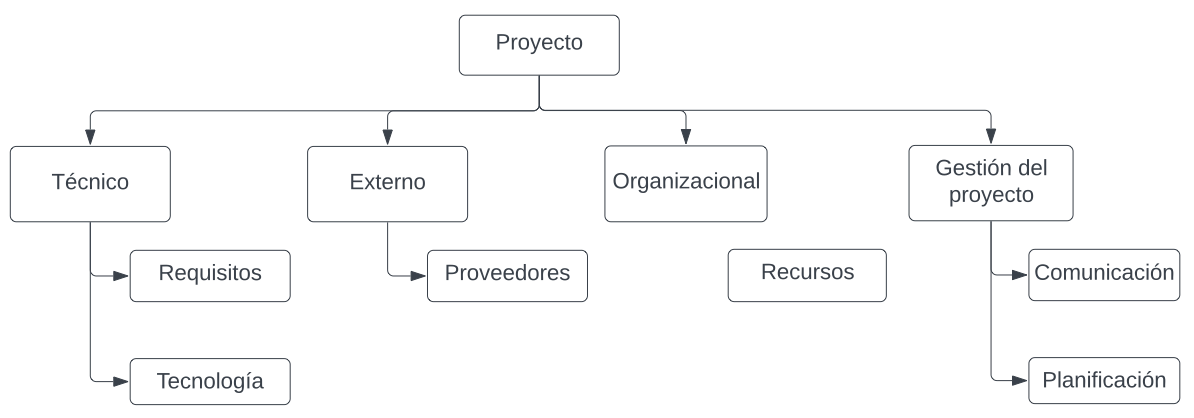
\includegraphics[scale=1.2]{rbs}}
\caption{Risk Breakdown Structure}
\end{figure}

\paragraph*{Probabilidad e impacto}
Se deben priorizar los riesgos de un proyecto en función de su prioridad de ocurrencia e impacto. A continuación se muestra la definición de las probabilidades y las escalas de impacto para riesgos negativos.
\begin{figure}[H]
\centering
\centerline{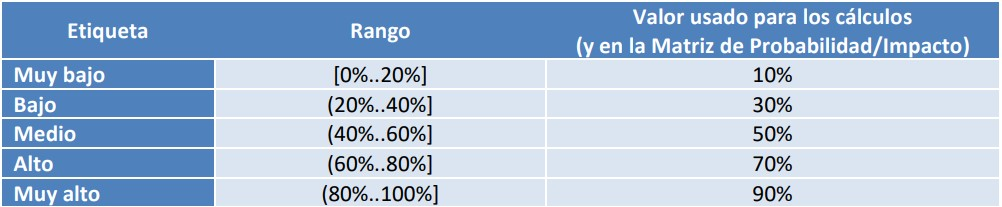
\includegraphics[scale=0.5]{def-probabilidades}}
\caption{Tabla de definición de probabilidades}
\end{figure}
\begin{figure}[H]
\centering
\centerline{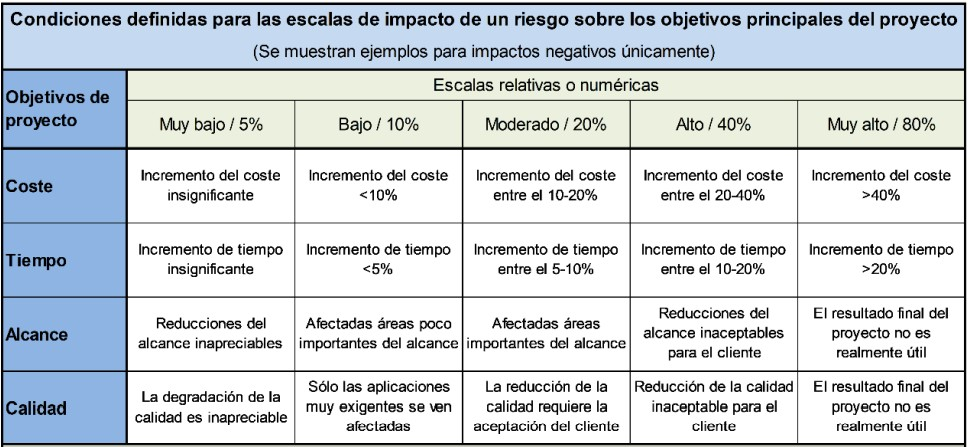
\includegraphics[scale=0.6]{escalas-impacto}}
\caption{Escalas de impacto sobre los objetivos del proyecto}
\end{figure}

\paragraph*{Matriz de probabilidad e impacto}
Esta matriz define los valores usados para priorizar los riesgos.
\begin{figure}[H]
\centering
\centerline{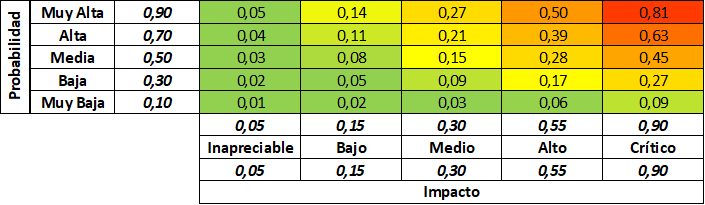
\includegraphics[scale=0.8]{matriz-prob}}
\caption{Matriz de Probabilidad e Impacto}
\end{figure}

\paragraph*{Estrategias de riesgo}
Para afrontar riesgos negativos se definen cuatro estrategias:
\begin{itemize}
\item Eliminar el riesgo.
\item Mitigar el riesgo.
\item Asumir el riesgo.
\item Transferir el riesgo.
\end{itemize}
Hay otras cuatro para riesgos positivos u oportunidades:
\begin{itemize}
\item Aprovechamiento.
\item Mejora.
\item Compartición.
\item Aceptación.
\end{itemize}


\newpage
\section{CONTENIDO ENTREGADO EN LOS ANEXOS}\label{sec:contenido_anexos}
%\addcontentsline{toc}{section}{CONTENIDO ENTREGADO EN LOS ANEXOS}

\subsection{Contenidos} 


Además de este documento, se hace entrega de una carpeta comprimida ``.zip'' en la que ahora se describirán sus contenidos. Se estructurará también la organización del código fuente.
\begin{itemize}
	\item \textbf{WBS.mpp} \(\rightarrow\) Archivo de Microsoft Project que contiene la planificación inicial del proyecto.
	\item \textbf{Presupuesto\_inicial.xlsx} \(\rightarrow\) Archivo Microsoft Excel que contiene los cálculos del presupuesto inicial del proyecto.
	\item \textbf{Presupuesto\_final.xlsx} \(\rightarrow\) Archivo Microsoft Excel que contiene los cálculos del presupuesto final del proyecto.
	\item \textbf{Informe\_Riesgos.xlsx} \(\rightarrow\) Archivo Microsoft Excel con el cálculo de probabilidad e impacto de los riesgos del proyecto.
	\item \textbf{Documentación\_Compodoc} \(\rightarrow\) Carpeta que contiene la documentación de los proyectos (museo y administración) generada con Compodoc. Abriendo el archivo \textit{index.html} de cada una de ellas se muestra la documentación correspondiente.
	\begin{itemize}
		\item \textbf{Documentación\_Museo} \(\rightarrow\) Contiene la documentación del proyecto del museo (museo-eii).
		\item \textbf{Documentación\_Admin} \(\rightarrow\) Contiene la documentación del proyecto de la administración del museo (museo-eii-admin).
	\end{itemize}
 	Cada una de estas carpetas contiene los archivos HTML con la documentación generada. Abriendo el archivo \textit{index.html} de cada una se puede ver la documentación al completo de su respectivo proyecto.
	\item \textbf{Diagramas} \(\rightarrow\) Carpeta que contiene todos los diagramas utilizados en este documento.
	\begin{itemize}
		\item \textit{Diagrama\_arquitectura\_tecnologica.png}
		\item \textit{Diagrama\_casos\_uso\_museo.png}
		\item \textit{Diagrama\_casos\_uso\_admin.png}
		\item \textit{Diagrama\_clases\_museo-Analisis.png}
		\item \textit{Diagrama\_clases\_admin-Analisis.png}
		\item \textit{Diagrama\_navegabilidad\_museo.png}
		\item \textit{Diagrama\_navegabilidad\_admin.png}
		\item \textit{Diagrama\_clases\_museo-Diseño.png}
		\item \textit{Diagrama\_clases\_admin-Diseño.png}
		\item \textit{Diagrama\_paquetes.png}
		%\item \textit{Diagrama\_componentes.png}
		\item \textit{Diagrama\_despliegue.png}
		\item \textit{Diagrama\_E-R.png}
	\end{itemize}
	\item \textbf{Codigo.zip} \(\rightarrow\) Carpeta comprimida con todo el código fuente. Está dividida a su vez en tres carpetas:
	\begin{itemize}
		\item \textbf{museo-eii} \(\rightarrow\) Contiene el proyecto de la aplicación del museo.
		\item \textbf{museo-eii-admin} \(\rightarrow\) Contiene el proyecto de la administración del museo.
		\item \textbf{back-end} \(\rightarrow\) Contiene los archivos PHP necesarios para conectarse con la base de datos del sistema, así como el script de creación de la base de datos e inserción de los datos iniciales. También tiene una carpeta \textit{upload}, con las imágenes de los componentes insertados a través del script.
	\end{itemize}
	museo-eii y museo-eii-admin tienen la misma estructura en su contenido. Ambas carpetas contienen:
	\begin{itemize}
		\item Carpeta \textbf{dist}: contiene los archivos necesarios para la distribución del proyecto.
		\item Carpeta \textbf{src}: contiene el código fuente del proyecto.
		\item \textbf{src/assets}: contiene las imágenes utilizadas en la aplicación y los archivos de internacionalización.
		\item \textbf{src/app}: contiene las clases (carpeta classes), los servicios (carpeta services) y los componentes de la aplicación (cada uno de ellos con su propia carpeta). Cada uno de estos elementos es un archivo \textit{.ts} donde se encuentra la funcionalidad correspondiente, al que acompaña un archivo \textit{.spec.ts} con las pruebas unitarias. Además los componentes también tienen asociados un archivo HTML y otro CSS para su visualización.
	\end{itemize} 
\par Se incluye un archivo \textit{README.md} con las instrucciones para la ejecución de ambos proyectos.
\end{itemize}